\section{Entrelacement des threads}

Les traces simulées sont générées par \textsf{MAQAO}, elles représentent une suite linéaire d'instructions. Elles ne reflètent donc pas le comportement réel de l'exécution parallèle du programme où les instructions sont réparties entre les différents c\oe urs du processeur. Ainsi, il faut choisir la manière d'exécuter séquentiellement ces instructions.

\subsection{Nécessité de l'entrelacement}

Sur une architecture multi-c{\oe}ur, plusieurs threads sont exécutés à la fois. Les threads exécutent donc des instructions en parallèle permettant ainsi d'augmenter la vitesse de calcul. Le problème est qu'il est possible de savoir sur quel c\oe ur une instruction a été exécutée, mais pas sa position dans l'exécution global du programme. En pratique les threads exécutent un certain nombre d'instructions avant de rendre la main, parfois en parallèle, et l'entrelacement réel des instructions dépend du programme, de l'OS, des interruptions, du matériel, \emph{etc}. L'ordre réel des instructions pendant une exécution n'est donc pas déterministe.\\

Le simulateur dispose d'une trace par coeur, et doit choisir combien d'instructions exécuter dans chaque trace avant de passer à une autre. Ce choix a une réelle influence sur les résultats de la simulation : il existe une cohérence entre les données utilisées par les différents c\oe urs et par conséquent lorsqu'un c\oe ur exécute une instruction, il devra aller chercher la donnée plus ou moins loin dans la hiérarchie selon si un autre c\oe ur l'a récemment chargée ou modifiée. \\

Il y a deux cas extrêmes :

\begin{itemize}
  \item \textbf{Lecture séquentielle} des traces de chaque thread l'une après l'autre. Supposons qu'un long calcul sur un tableau soit partagé par deux threads : les données utilisées au début du calcul par le premier thread ne seront peut-être plus présentes dans les caches à la fin du calcul et le second thread aura besoin de les recharger plus loin dans la mémoire pour les lire. On peut noter que ce cas met au second plan la gestion de la cohérence des données, qui influe peu sur le résultat.
  \item \textbf{Lecture une par une} des instructions, en changeant de thread à chaque fois. Cela permet de mieux préserver la localité temporelle. Les ressources partagées par deux threads auront plus de chances d'être lues et écrites par différents threads et la cohérence des données prend une plus grande importance.
\end{itemize} 

Ces deux cas ne sont pas réalistes, mais sont néanmoins intéressants pour évaluer les comportements les plus critiques en théorie.\\


Un modèle de base a été implémenté afin de configurer l'ordre d'exécution des traces, appelé entrelacement des threads. Celui choisi pour le simulateur fonctionne de la manière suivante : un certain nombre d'instructions sont exécutées sur un thread, une fois terminées ce sont autant d'instructions qui sont exécutées sur le c\oe ur suivant. Cela revient à rendre le programme  séquentiel en entrelaçant les instructions sur les différents threads.

\subsection{Entrelacement bloc par bloc}

Le choix d'entrelacement par défaut qui a été fait permet donc de changer de c\oe ur sur lequel il faut exécuter les instructions de manière cyclique entre les c\oe urs, toutes les $x$ instructions, $x$ étant la taille choisie pour les blocs d'instructions. La figure \ref{img:entrelacement} explicite visuellement quand sont exécutées les instructions par blocs, numérotés par ordre de lecture. La technologie utilisée est un script \texttt{LUA} qui retourne le prochain coeur sur lequel le simulateur doit exécuter les instructions. Ce script permet de fixer un nombre d'instructions à exécuter avant de changer de coeur, pour changer de coeur à chaque instruction il faut donc réduire la taille du bloc d'instructions à exécuter à une seule instruction.\\

\begin{figure}[!h]
\begin{center}
   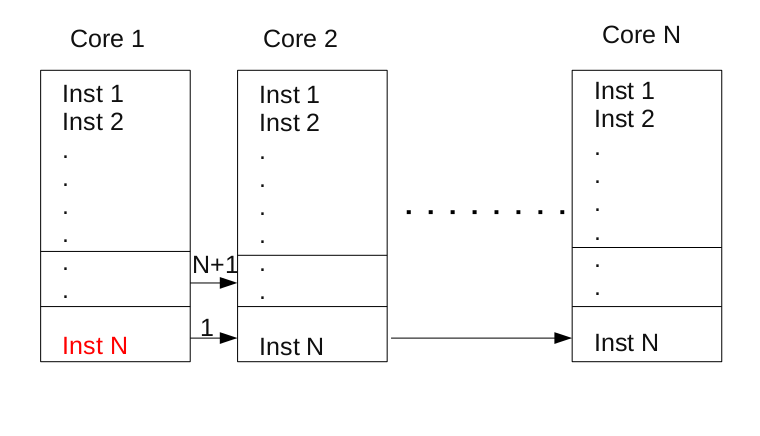
\includegraphics[width=0.8\textwidth]{images/entrelacement.png}
   \caption{\label{img:entrelacement} Ordre d'exécution de blocs de taille trois instructions, de chaque trace/c\oe ur.}
\end{center}
\end{figure}



Le modèle d'entrelacement des threads étant placé dans un fichier LUA, celui-ci est modifiable sans nouvelle compilation. Dans le cas où les traces n'ont pas toutes le même nombre d'instructions, il n'est toutefois pas possible depuis le script de savoir si une trace est terminée alors que les autres non. Si le c\oe ur renvoyé par le script n'a plus d'instruction à lire sur la trace associée, rien ne se produira, et le script renverra le c\oe ur suivant. 

